\chapter{Supplementary Material for Contribution 1 (RQ1)}\label{app:rq1}

\section{Nomenclature}

Table~\ref{tab:nomenclature_rq1} lists the complete nomenclature for the fast-charging infrastructure allocation model described in Section~\ref{sec:rq1_results}.

\begin{scriptsize}
\begin{longtable}{llll}
\caption{Nomenclature for the fast-charging infrastructure allocation model (RQ1).}
\label{tab:nomenclature_rq1}\\
\hline
Sets and indices & Description & & \\ \hline
\endfirsthead
\endhead
\hline
\endfoot
\endlastfoot
$n, l \in \{0, \dots, N\}$ & node index & & \\
$k \in \{0, 1\}$ & driving direction & & \\
$s \in \{0, \dots, M\}$ & highway segment index & & \\
$A_{n_k}$ & \begin{tabular}[t]{@{}l@{}}set of nodes accessible within\\ $dist_{max}$ from node $n$ in direction $k$\end{tabular} & & \\
\\\hline
Decision variables & Description & Unit & Type / Domain \\ \hline
$X_{l}$ & \begin{tabular}[t]{@{}l@{}}whether a charging station is\\ installed at node $l$\end{tabular} & -- & $\{0, 1\}$ (binary) \\
$Y_{l_k}$ & \begin{tabular}[t]{@{}l@{}}number of charging points\\ at node $l_k$\end{tabular} & -- & $\mathbb{Z}_{\geq 0}$ (integer) \\
$\hat{E}_{l_k}^{charged, n_k}$ & \begin{tabular}[t]{@{}l@{}}charged energy at node $l_k$\\ of demand from node $n_k$ during peak hour\end{tabular} & kWh/h & $[0, \infty[$ \\
$\hat{D}_{l_k}^{in, n_k}$ & \begin{tabular}[t]{@{}l@{}}energy demand from node $n_k$,\\ incoming to node $l_k$ during peak hour\end{tabular} & kWh/h & $[0, \infty[$ \\
$\hat{D}_{l_k}^{out, n_k}$ & \begin{tabular}[t]{@{}l@{}}energy demand from node $n_k$, not\\ covered and outgoing from $l_k$ during peak hour\end{tabular} & kWh/h & $[0, \infty[$ \\
\\\hline
Parameters -- car fleet & Description & Unit & Domain \\ \hline
$\epsilon$ & share of BEVs in total passenger car fleet & \% & $[0, 1]$ \\
$\mu$ & share of cars traveling long-distance & \% & $[0, 1]$ \\
$\gamma_h$ & \begin{tabular}[t]{@{}l@{}}share of daily car count traveling\\ during peak hour\end{tabular} & \% & $[0, 1]$ \\
$\hat{f}_{n_k}$ & \begin{tabular}[t]{@{}l@{}}maximum daily amount of cars passing\\ at node $n$ in direction $k$ during a year\end{tabular} & 1/24h & $[0, \infty[$ \\
$\alpha$ & \begin{tabular}[t]{@{}l@{}}share of overall road traffic load compared\\ with year of survey of traffic counts\end{tabular} & \% & $[0, \infty[$ \\
\\\hline
Parameters -- BEV technology & Description & Unit & Domain \\ \hline
$\overline{d}_{spec, BEV}$ & \begin{tabular}[t]{@{}l@{}}average specific energy demand\\ per km of BEVs\end{tabular} & kWh/km & $[0, \infty[$ \\
$\overline{dist}_{range, BEV}$ & average driving range of BEVs & km & $[0, \infty[$ \\
$\overline{P}_{charge, BEV}$ & average charging capacity of BEVs & kW & $[0, \infty[$ \\
\\\hline
Parameters -- infrastructure & Description & Unit & Domain \\ \hline
$\hat{P}_{CP}$ & peak power level of a charging point & kW & $[0, \infty[$ \\
$P_{max}$ & \begin{tabular}[t]{@{}l@{}}maximum capacity installed\\ at a charging station\end{tabular} & kW & $[0, \infty[$ \\
$c_{X}$ & \begin{tabular}[t]{@{}l@{}}investment costs for installation\\ of a charging station\end{tabular} & EUR & $[0, \infty[$ \\
$c_{Y}$ & \begin{tabular}[t]{@{}l@{}}investment costs for installation\\ of one charging point\end{tabular} & EUR & $[0, \infty[$ \\
\\\hline
Derived parameters & Description & Unit & Domain \\ \hline
$dist_{ns_k}$ & \begin{tabular}[t]{@{}l@{}}distance of node $n$ along\\ segment $s$ in direction $k$\end{tabular} & km & $[0, \infty[$ \\
$GRNN_{s_k}(dist)$ & \begin{tabular}[t]{@{}l@{}}GRNN function of peak daily traffic\\ load along segment $s$ in direction $k$\end{tabular} & -- & $[0, \infty[$ \\
$\hat{D}_{n_k}$ & \begin{tabular}[t]{@{}l@{}}average energy demand at node $n$\\ in direction $k$ during peak hour\end{tabular} & kWh/h & $[0, \infty[$ \\
$dist_{max}$ & \begin{tabular}[t]{@{}l@{}}maximum distance between\\ charging stations\end{tabular} & km & $[0, \infty[$ \\
$r_{l_k, l_k'}$ & \begin{tabular}[t]{@{}l@{}}rationing parameter for demand\\ flow split at junction nodes\end{tabular} & -- & $[0, 1]$ \\
\hline
\end{longtable}
\end{scriptsize}

\section{Computational Details}

The optimization model is implemented in Python~3.8 using Pyomo~6.2 as the algebraic modeling language and Gurobi~9.1.2 as the solver. The Austrian highway network is represented by 249 nodes (139 service areas and 110 junctions) along 55 highway segments. Depending on the assumed BEV driving range, the resulting mixed-integer linear program comprises approximately 1.3~million constraints. Solve times range from 650~seconds (at a driving range of 400~km) to 1{,}360~seconds (at 800~km), with a maximum optimality gap (MIPgap) of 0.2\%.

The source code and input data are publicly available at: \url{https://github.com/antoniagolab/HighCharge}.

\section{Determination of Average Technological Parameters for BEVs}\label{app:rq1_bev_params}

To evaluate the technological parameters of an average battery-electric vehicle (BEV) in the Austrian car fleet, the technological attributes of the most sold car models from the last three years were used. These are displayed in Table~\ref{tab:top10_rq1} with the respective number of sales. Using sale numbers as weights, the weighted averages for the driving range and charging capacity were evaluated.

\begin{table}[H]
\begin{adjustwidth}{-\extralength}{0cm}
\caption{Top 10 sold car models in Austria in 2019--2021 and technical attributes \citep{statista1920, statista21, evdb} (average driving range $\overline{dist}_{range,BEV}$, average charging power $\overline{P}_{charge,BEV}$, average specific energy demand $\overline{d}_{spec,BEV}$).}\label{tab:top10_rq1}
\resizebox{18.5cm}{!}{%
\begin{tabular}{@{}lcccccc@{}}
\toprule
Car model                        & Sales 2019 & Sales 2020 & Sales 2021 & $\overline{dist}_{range,BEV}$ $(km)$ & \begin{tabular}[c]{@{}c@{}} $\overline{P}_{charge,BEV}$\\ at $\hat{P}_{CP}= 150kW$\\ $(kW)$\end{tabular} & \begin{tabular}[c]{@{}c@{}}$\overline{d}_{spec,BEV}$ \\ highway - cold weather\\ $(kWh/km)$\end{tabular} \\ \midrule
\textit{Tesla Model 3}           & 2342       & 2892       & 3304       & 380                     & 110                                                                                                   & 0.23                                                                                            \\
\textit{Renault Zoe}             & 944        & 2071       & 1778       & 310                     & 41                                                                                                    & 0.22                                                                                            \\
\textit{Kia Niro}                & 1125       & 421        & 924        & 370                     & 77                                                                                                    & 0.24                                                                                            \\
\textit{Hyundai Kona}            & 897        & 861        & -          & 395                     & 64                                                                                                    & 0.28                                                                                            \\
\textit{Audi e-Tron}             & 364        & 782        & 1192       & 285                     & 114                                                                                                   & 0.29                                                                                            \\
\textit{BMW i3}                  & 1191       & 697        & -          & 235                     & 47                                                                                                    & 0.23                                                                                            \\
\textit{VW e-Golf}               & 805        & 401        & -          & 190                     & 39                                                                                                    & 0.24                                                                                            \\
\textit{VW Up!}                  & -          & 376        & -          & 205                     & 30                                                                                                    & 0.22                                                                                            \\
\textit{Mazda MX-30}             & -          & 370        & -          & 170                     & 34                                                                                                    & 0.25                                                                                            \\
\textit{Peugeot 208}             & -          & 355        & -          & 285                     & 78                                                                                                    & 0.23                                                                                            \\
\textit{Hyundai Ioniq}           & 361        & -          & -          & 250                     & 36                                                                                                    & 0.22                                                                                            \\
\textit{Nissan Leaf}             & 557        & -          & -          & 225                     & 40                                                                                                    & 0.23                                                                                            \\
\textit{Tesla Model S}           & 389        & -          & -          & 560                     & 110                                                                                                   & 0.23                                                                                            \\
\textit{VW ID.3}                  & -          & -          & 2361       & 350                     & 85                                                                                                    & 0.23                                                                                            \\
\textit{VW ID.4}                  & -          & -          & 2361       & 400                     & 103                                                                                                   & 0.27                                                                                            \\
\textit{Skoda Enyaq}             & -          & -          & 2208       & 420                     & 103                                                                                                   & 0.26                                                                                            \\
\textit{Fiat 500}                & -          & -          & 1356       & 235                     & 67                                                                                                    & 0.23                                                                                            \\
\textit{Seat Mii}                & -          & -          & 936        & 205                     & 30                                                                                                    & 0.22                                                                                            \\
\textit{Tesla Model Y}           & -          & -          & 921        & 435                     & 108                                                                                                   & 0.24                                                                                            \\ \midrule
\textbf{Weighted average values} &            &            &            & \textbf{340}            & \textbf{81}                                                                                           & \textbf{0.24}                                                                                   \\ \bottomrule
\end{tabular}%
}
\end{adjustwidth}
\end{table}

\section{Details on Projected Developments for 2030}\label{app:rq1_projections}

For the quantification of the scenarios used in the analysis, projections on the development of BEV share had to be made. For the \textit{Societal Commitment} and \textit{Techno-Friendly} scenarios an \textit{optimistic} projection was made based on the decarbonization goals for the transport sector in the governmental document \enquote{Austria's Mobility Master Plan 2030} \citep{Nachhaltig}. A \textit{pessimistic} projection is made for the \textit{Directed Transition} and \textit{Gradual Development} scenarios based on the trend of new registrations of BEVs in the years between 2018 and 2020.

\begin{figure}[H]
\centering
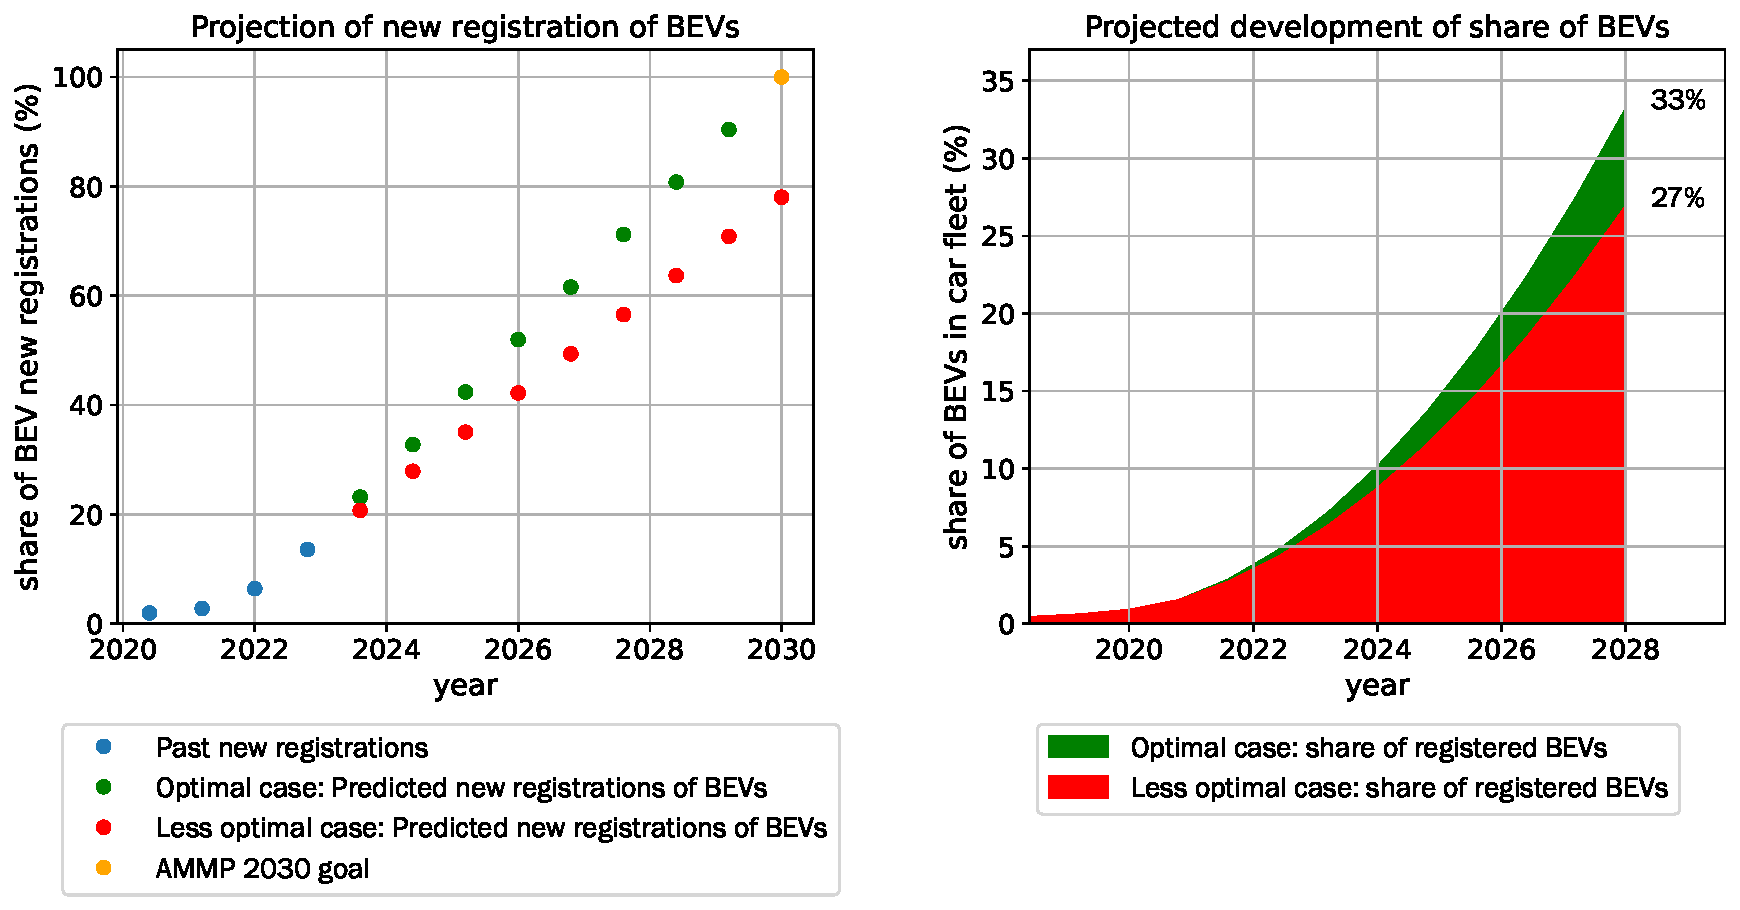
\includegraphics[width=14cm]{graphics/paper_1/appendix_img_meth.pdf}
\caption{Projections of linearly increasing new registrations of BEVs (\textbf{left}, \textit{AMMP}=\textit{Austria Mobility Master Plan} \citep{Nachhaltig}) and based on this, developments of the share of BEVs (\textbf{right}).}\label{fig:bev_pen_proj}
\end{figure}

\section{Details on Data Preparation for the Austrian Case Study}\label{app:rq1_data_prep}

The underlying data pre-processing procedures of this work encompassed the preparation of the graph representation of the Austrian high-level road network and the potential sites for the installment of charging stations. Geographic data representing the Austrian highways and motorways was obtained based on OpenStreetMap data \cite{OpenStreetMap}. For this, all \textit{way} instances with tags \textit{highway=`motorway'} and \textit{highway=`trunk'} were retrieved and further processed using ArcGIS Pro \cite{desktop2011release} in order to obtain a clean shape representation of the road network, including the representation of both driving directions through parallel lines. Geographic data implying positions of service areas were retrieved using tags \textit{highway=`services'} and \textit{highway=`rest\_area'}. This geographic information was paired with data on service areas obtained through ASFINAG \cite{asfinagrastanlagen} which provide information on the driving direction a service area is accessible from and on the services offered on-site.
